% !TEX root = ../../../under-spec-z.tex

\subsection{Background knowledge} % (fold)
\label{sub:background_knowledge}

    This section acts as a prelude to \cite{Toen:2005wxa}, containing a few motivating examples and prerequisite definitions and lemmas.
    Before diving straight into the abstract definitions, we give an example of why we might think to try a category-theoretic approach to algebraic geometry.

    \subsubsection{Motivating example} % (fold)
    \label{ssub:motivating_example}

        Let $A$ be a finitely-generated commutative $k$-algebra.
        Then we can write
        \begin{equation*}
            A=\frac{k[x_1,\ldots,x_n]}{(f_1,\ldots,f_m)}
        \end{equation*}
        for some $m,n\in\nn$ and $f_i\in k[x_1,\ldots,x_n]$.
        If $B$ is another commutative $k$-algebra (not necessarily finitely generated) then the collection of algebra morphisms $A\to B$ is in bijection with points of $B^n$ that vanish on all of the $f_i$, since a morphism is determined entirely by where it sends each of the $x_i$ whilst satisfying $0\mapsto0$.
        So, letting $\commk$ denote the category of commutative $k$-algebras,
        \begin{equation}\label{eq:link-between-hom-and-varieties}
            \Hom_{\commk}(A,B)\cong\{b\in B^n \mid f_1(b)=\ldots=f_m(b)=0\}
        \end{equation}
        where, as usual, we evaluate $f_i(b)$ inside $B$.

        \Cref{eq:link-between-hom-and-varieties} implies that we should maybe think of $\Hom(A,B)$ as some variety inside $B^n$ determined by $A$, for general $A,B\in\commk$, and so we might be able to recover a lot of algebraic geometry from studying these $\Hom(A,B)$.
        In fact, thinking of $\Hom(A,\blank)$ as a functor $\commk\to\Set$ which takes an algebra $B$ to a \emph{variety} (a set of points) inside $B^n$, we are led to the more general idea of studying \emph{all} functors $\commk\to\Set$, and calling such functors \emph{spaces}.

        Before formalising this, we first recall a few things from category theory.
        
        \begin{definition}[Presheaves]\label{df:presheaves}
            Let $\ccat$ be a category.
            The category of \emph{presheaves on $\ccat$} is defined as the functor category $\PShv(\ccat)=\Fun(\op{\ccat},\Set)$, whose objects are (covariant) functors $\op{\ccat}\to\Set$ and morphisms are natural transformations $F\nt G$ between such functors.
        \end{definition}

        % \begin{figure}[h]
        %     \centering
        %     \frame{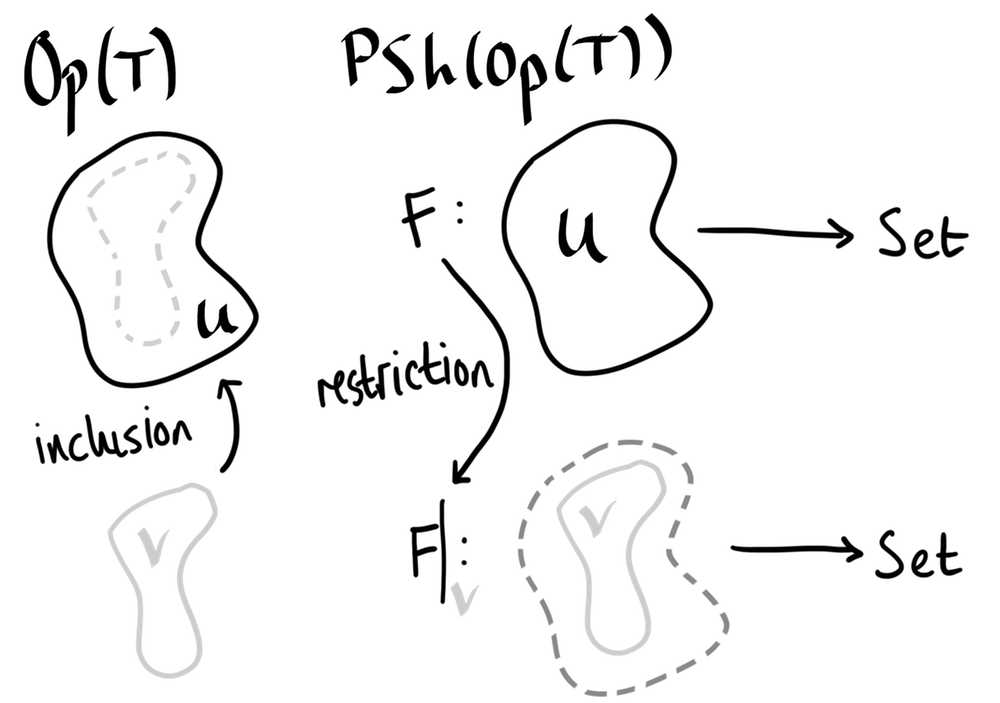
\includegraphics[width=.6\textwidth]{images/presheaves.png}}
        %     \caption{Presheaves on $\Op{T}$ (see paragraph after \cref{df:pullbacks}) -- inclusion of open sets corresponds to restriction of presheaves}
        %     \label{fg:presheaves}
        % \end{figure}

        \begin{figure}[h]
            \centering
            \frame{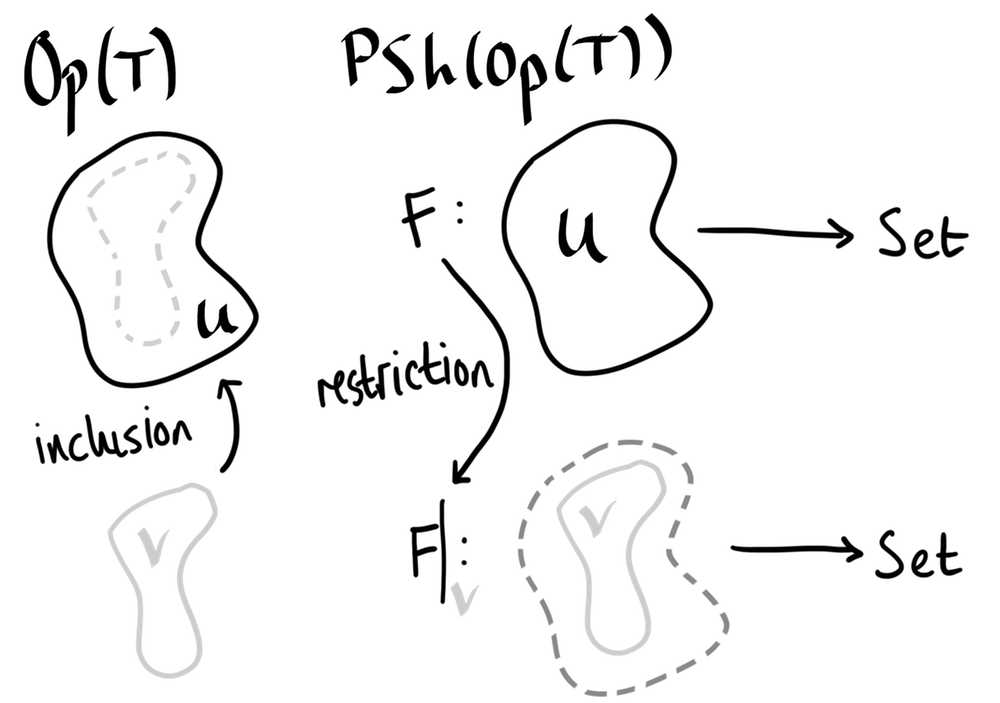
\includegraphics[width=.63\textwidth]{images/presheaves.png}}
            \caption{Presheaves on $\Op{T}$ (see paragraph after \cref{df:pullbacks}) -- inclusion of open sets corresponds to restriction of presheaves}\label{fg:presheaves}
        \end{figure}

        \begin{lemma}[Yoneda lemma]\label{le:yoneda-lemma}
            Let $\ccat$ be a locally small category\footnote{
                That is, the hom-sets $\Hom(A,B)$ are actual sets for all $A,B\in\ccat$.
            }.
            Define the \emph{downwards Yoneda functor}\footnote{
                This is not at all common terminology.
                It is often called the \emph{contravariant Yoneda functor}: it maps an object $A\in\ccat$ to the \emph{contravariant} functor $\Hom_\ccat(\blank,A)\colon\ccat\to\Set$.
                But the functor $\ccat\to\PShv(\ccat)$ itself is \emph{covariant}, so we use `downwards' to avoid confusion.
                The dual `covariant' (\emph{upwards}, in our terminology) functor is $Y^{(\blank)}\colon\op{\ccat}\to\Fun(\ccat,\Set)$ given by $\spec A\mapsto Y^A=\Hom_\ccat(A,\blank)$, where we write $\spec A\in\op{\ccat}$ to be the object corresponding to $A\in\ccat$.
                Then the statement $\Hom_{\Fun(\ccat,\Set)}(Y^A,G)\cong G(A)$ holds.
            } by
            \begin{align*}
                Y_{(\blank)}\colon&\ccat\to\PShv(\ccat)\\
                &A\mapsto \Hom_\ccat(\blank, A),
            \end{align*}
            which is well defined, since $\Hom(\blank, A)\colon\op{\ccat}\to\Set$ covariantly.
            Then, for any $A\in\ccat$ and $F\in\PShv(\ccat)$,
            \begin{equation}
                \Hom_{\PShv(\ccat)}(Y_A,F) \cong F(A)
            \end{equation}
            via the canonical restriction map.
            Further, $Y$ is fully faithful.
        \end{lemma}

        \begin{proof}
            See \cite[\S III.2, p.59--62]{Lane:1998fe}.
        \end{proof}

        Since $\commk$ is locally small\footnote{
            As in \cite{Toen:2005wxa}, we try to ignore such set-theoretic issues, but here we have the reasonable explanation that $\commk$ is a concrete category, and thus locally small.
        }, we can make the definitions in \cref{tb:comm-k-definitions}, where $Y$ is the Yoneda functor from \cref{le:yoneda-lemma}\footnote{
            In the definition of $\spec$ we use the fact that any covariant functor $F\colon\ccat\to\dcat$ induces a contravariant functor $F\colon\op{\ccat}\to\dcat$, and vice versa.
        }.
        
        \bigskip
        \begin{table}[h!]
            \centering
            \begin{tabular}{lcc}
                Name & Notation & Definition\\
                \toprule
                the category of \emph{affine schemes over $k$} & $\aff{k}$ & $\op{\commk}$\\
                the category of \emph{$k$-spaces} & $\Sp{k}$ & $\PShv(\aff{k})$\\
                the \emph{spectrum functor} & $\spec$ & $Y\colon\commk\to\Sp{k}$
            \end{tabular}
            \caption{Categorical approach to algebraic geometry with $\commk$}
            \label{tb:comm-k-definitions}
        \end{table}
        \bigskip

        We've already given a reason for calling objects of the functor category $\Fun(\commk,\Set)$ \emph{spaces}, and we call objects of $\op{\commk}$ \emph{schemes} because we know that the Yoneda lemma (\cref{le:yoneda-lemma}) will give us a way of viewing $\aff{k}$ as sitting inside of $\Sp{k}$.

        \begin{lemma}[Yoneda embedding]\label{le:yoneda-embedding}
            The category $\aff{k}$ is equivalent to the essential image of the Yoneda functor $Y\colon\aff{k}\to\Sp{k}$.
        \end{lemma}

        \begin{proof}
            Here we use the fact that a functor gives an equivalence of categories if and only if it is fully faithful and essentially surjective\footnote{
                \cite[Theorem~1, \S IV.4]{Lane:1998fe}
            }.
            \cref{le:yoneda-lemma} tells us that $Y$ is fully faithful so it forms an equivalence of categories between $\aff{k}$ and the essential image of $Y$ in $\Sp{k}$.
        \end{proof}

        So \cref{le:yoneda-embedding} lets us imagine $\aff{k}$ as sitting inside $\Sp{k}$.
        This mirrors classical algebraic geometry where, loosely speaking, given some commutative ring $R$ we define the space $\spec R$ of prime ideals of $R$ endowed with the Zariski topology.
        We can then give $\spec R$ some extra structure to make it an affine scheme.
        Then $\spec$ is a map taking commutative rings to affine schemes, which form a subclass of the objects (schemes) in which we're interested.

        Studying algebraic geometry this way is called the \emph{functor of points} approach\footnote{
            As opposed to the traditional \emph{ringed space} approach.
        }, because \cref{le:yoneda-embedding} says that describing some affine scheme $X\in\aff{k}$ is exactly the same as describing its functor of points $X(\blank)\in\Sp{k}$ under the Yoneda embedding.
        Sometimes this latter method is far easier, as the following example shows.

        \begin{example}[$\GL_n$]\label{ex:gln-affine-scheme}
            Given $A\in\commk$ we can define $\GL_n(A)$ to be the group of $n\times n$ invertible matrices over $A$.
            This induces a functor $\GL_n(\blank)\colon\op{\aff{k}}\to\Set$, so $\GL_n(\blank)\in\Sp{k}$.
            We claim that this functor is in the essential image of the Yoneda (spectrum) functor $Y\colon\commk\to\Sp{k}$, and is thus represented by an affine scheme.
            This is not obvious a priori.
            To prove this, we need to find an isomorphism
            \begin{equation*}
                \GL_n(\blank)\cong\Hom_{\commk}(R,\blank)=\spec R
            \end{equation*}
            for some $R\in\commk$, where we mean $\spec R$ as defined in \cref{tb:comm-k-definitions}\footnote{
                That is, identify $\spec R\in\aff{k}$ with $\spec R:=\Hom_{\op{\commk}}(\blank,R)$.
            }.
            By definition, this is equivalent to finding a bijection of sets $\GL_n(A)\cong\Hom_{\commk}(R,A)$ that transforms naturally in $A$ for each $A\in\commk$.

            Note that an element of $\GL_n(A)$ is a choice of $x_{11},x_{21},\ldots,x_{nn}\in A$ such that $\det(x_{ij})$ is invertible.
            That is, there exists some $y\in A$ such that $y\det(x_{ij})=1$.
            Hence
            \begin{equation*}
                R=\frac{k[x_{11},x_{21},\ldots,x_{nn},y]}{(y\det(x_{ij})-1)}
            \end{equation*}
            gives us the desired result, and so $GL_n=R\in\aff{k}$ is an affine scheme.
        \end{example}

    % subsubsection motivating_example (end)


    \subsubsection{Preliminary definitions} % (fold)
    \label{ssub:preliminary_definitions}

        We now give some definitions of which \cite{Toen:2005wxa} assumes prior knowledge.
        The motivation for them usually comes from taking $\ccat=\Set$, and their application to algebraic geometry can be better understood\footnote{
            Since \emph{\elide a commutative ring is nothing but a commutative monoid in the monoidal category of $\zz$-modules \elide} (\S1 p.2 \P1).
        } by taking $\ccat=\modc{\zz}=\Ab$.
        We assume that the reader is familiar with notions such as categories, functors, natural transformations, and functor categories, but not too much else.

        \begin{definition}[Monoidal category]\label{df:monoidal-category}
            A \emph{monoidal category} consists of the following data:
            \begin{itemize}
                \item a category $\ccat$;
                \item an object $1\in\ccat$, which we call the \emph{unit} or \emph{identity};
                \item a bifunctor $(\blank\otimes\blank)\colon\ccat\times\ccat\to\ccat$, called the \emph{monoidal} or \emph{tensor product};
                \item natural isomorphisms $\alpha$ (the \emph{associator}), $\lambda$ (the \emph{left unitor}), and $\rho$ (the \emph{right unitor}), constructed from morphisms
                \begin{equation*}
                    \begin{array}{rrcl}
                        \alpha_{ABC}\colon & (A\otimes B)\otimes C & \congto & A\otimes(B\otimes C)\\
                        \lambda_A\colon & 1\otimes A & \congto & A\\
                        \rho_A\colon & A\otimes1 & \congto & A
                    \end{array}
                \end{equation*}
                for all $A,B,C\in\ccat$.
            \end{itemize}
            Further, the three natural isomorphisms are subject to the following coherence conditions\footnote{
                These diagrams simply say that $\otimes$ is associative in all the ways that you might expect.
            }:
            \begin{itemize}
                \item (\emph{unit associativity}) for all $A,B\in\ccat$ the following commutes
                    \begin{equation*}
                        \begin{tikzcd}[row sep=3em]
                            (A\otimes 1)\otimes B \arrow[dr, swap, "\rho_A\otimes\id_B"] \arrow[rr, "\alpha_{A1B}"] & & A\otimes(1\otimes B) \arrow[dl, "\id_A\otimes\lambda_B"]\\
                             & A\otimes B &
                        \end{tikzcd}
                    \end{equation*}
                \item (\emph{4-associativity}) for all $A,B,C,D\in\ccat$ the following commutes
                    \begin{equation*}
                        \begin{tikzcd}[column sep=-3em, row sep=4em, cramped]
                            & (A\otimes(B\otimes C))\otimes D \arrow[rr, "\alpha_{A(B\otimes C)D}"] & & A\otimes((B\otimes C)\otimes D) \arrow[dr, "\id_A\otimes\alpha_{BCD}"] &\\
                            ((A\otimes B)\otimes C)\otimes D \arrow[ur, "\alpha_{ABC}\otimes\id_D"] \arrow[drr, "\alpha_{(A\otimes B)CD}", swap] & & & & A\otimes(B\otimes(C\otimes D)) \\
                             & & (A\otimes B)\otimes(C\otimes D) \arrow[urr, "\alpha_{AB(C\otimes D)}", swap] & &
                        \end{tikzcd}\qedhere
                    \end{equation*}
            \end{itemize}
        \end{definition}

        \begin{definition}[Symmetric monoidal category]\label{df:smc}
            A monoidal category $\smc$ is \emph{symmetric} if it can be equipped with a \emph{maximally-symmetric brading $\gamma$}.
            That is, for all $A,B\in\ccat$, there exists an isomorphism
            \begin{equation*}
                \gamma_{AB}\colon A\otimes B\congto B\otimes A
            \end{equation*}
            that is natural in both $A$ and $B$, and also subject to the following coherence conditions\footnote{
                These diagrams simply say that $\otimes$ is commutative in all the ways you might expect.
            }:
            \begin{itemize}
                \item (\emph{unit associativity}) for all $A\in\ccat$ the following commutes:
                    \begin{equation*}
                        \begin{tikzcd}
                            1\otimes A \arrow[rr, "\gamma_{1A}"] \arrow[dr, swap, "\lambda_A"] & & A\otimes 1 \arrow[dl, "\rho_A"]\\
                             & A &
                        \end{tikzcd}
                    \end{equation*}
                \item (\emph{3-associativity}) for all $A,B,C\in\ccat$ the following commutes:
                    \begin{equation*}
                        \begin{tikzcd}[column sep=4em,row sep=3em]
                            (A\otimes B)\otimes C \arrow[r, "\gamma_{AB}\otimes\id_C"] \arrow[d, swap, "\alpha_{ABC}"] & (B\otimes A)\otimes C \arrow[d, "\alpha_{BAC}"]\\
                            A\otimes(B\otimes C) \arrow[d, swap, "\gamma_{A(B\otimes C)}"] & B\otimes(A\otimes C) \arrow[d, "\id_B\otimes\gamma_{AC}"]\\
                            (B\otimes C)\otimes A \arrow[r, "\alpha_{BCA}"] & B\otimes(C\otimes A)
                        \end{tikzcd}
                    \end{equation*}
                \item (\emph{maximal symmetry}) for all $A,B\in\ccat$ the following commutes:
                    \begin{equation*}
                        \begin{tikzcd}
                             & B\otimes A \arrow[dr, "\gamma_{BA}"] & \\
                            A\otimes B \arrow[ur, "\gamma_{AB}"] \arrow[rr, swap, "\id_{A\otimes B}"] & & A\otimes B
                        \end{tikzcd}
                    \end{equation*}\qedhere
            \end{itemize}
        \end{definition}

        \begin{definition}[Closed symmetric monoidal category\footnote{ See \cite[Hypothese 2.6,~p.14]{Toen:2005wxa}}]\label{df:closed-smc}
            A symmetric monoidal category $\smc$ is \emph{closed} if, for all $A\in\ccat$, the functor $\blank\otimes A\colon\ccat\to\ccat$ has a right adjoint, written $(A\nt\blank)$.
            This means that
            \begin{equation*}
                \Hom(X\otimes A,B)\cong\Hom(X,A\nt B)
            \end{equation*}
            naturally in $X$ and $B$ for all $A,B,X\in\ccat$.
            The object $(A\nt B)\in\ccat$ is called the \emph{internal Hom}\footnote{
                \cite{Toen:2005wxa} uses the notation $\uHom(A,B)$.
            }.
        \end{definition}

        \begin{lemma}
            Let $\smc$ be a closed symmetric monoidal category.
            Then the bifunctor
            \begin{equation*}
                (\blank\otimes\blank)\colon\ccat\times\ccat\to\ccat
            \end{equation*}
            commutes with colimits in both of its arguments.
        \end{lemma}

        \begin{proof}
            % \emph{(We first show commutativity only in the first argument, and then explain at the end how to use this to complete the proof.)}

            % Fix $A\in\ccat$ and let $\{X_i\}_{i\in I}$ be a collection of objects in $\ccat$.
            % Assume that we have some $B\in\ccat$ with morphisms $X_i\otimes A\to B$ for all $i\in I$, and such that
            % \begin{equation}\label{eq:colim-commute-setup}
            %     \begin{tikzcd}[column sep=2em]
            %         X_i\otimes A \arrow[dr] \arrow[rr] & & X_j\otimes A \arrow[dl]\\
            %          & B &
            %     \end{tikzcd}
            % \end{equation}
            % commutes for all $X_i\otimes A\to X_j\otimes A$.
            % Then we want to show that there exists
            % \begin{itemize}
            %     \item morphisms $X_i\otimes A,X_j\otimes A\to(\colim X_i)\otimes A$;
            %     \item a \emph{unique} morphism $(\colim X_i)\otimes A\to B$,
            % \end{itemize}
            % such that the following diagram commutes:
            % \begin{equation}\label{eq:what-we-want-to-commute}
            %     \begin{tikzcd}[column sep=1em,row sep=2em]
            %         X_i\otimes A \arrow[dr] \arrow[ddr, bend right] \arrow[rr] & & X_j\otimes A \arrow[dl] \arrow[ddl, bend left]\\
            %          & (\colim X_i)\otimes A \arrow[d] &\\
            %          & B &
            %     \end{tikzcd}
            % \end{equation}

            % If we can show this, then, because the colimit is unique up to unique isomorphism\footnote{
            %     We write $X\overset{!}{\cong}Y$ to mean there these exists a \emph{unique} isomorphism between $X$ and $Y$.
            % },
            % \begin{equation*}
            %     (\colim X_i)\otimes A\overset{!}{\cong} \colim(X_i\otimes A).
            % \end{equation*}

            % \bigskip

            % This proof is largely diagram chasing, and it's easy to get lost in notation, but the idea behind it is comparatively simple: we construct four \emph{unique} morphisms that make certain diagrams commute, then put them all together.

            % \begin{enumerate}[(i)]

            %     \item \emph{Universal property of $\colim(X_i\otimes A)$}:

            %         By definition, there exists a unique $\pi\colon\colim(X_i\otimes A)\to B$ such that
            %         \begin{equation*}
            %             \begin{tikzcd}[column sep=1em,row sep=2em]
            %                 X_i\otimes A \arrow[dr] \arrow[ddr, bend right] \arrow[rr] & & X_j\otimes A \arrow[dl] \arrow[ddl, bend left]\\
            %                  & \colim(X_i\otimes A) \arrow[d, "\pi"] &\\
            %                  & B &
            %             \end{tikzcd}
            %         \end{equation*}
            %         commutes.

            %     \item \emph{Closedness of $\smc$ and universal property of $\colim X_i$}:

            %         \Cref{df:closed-smc} tells us that there is an isomorphism
            %         \begin{equation*}
            %             \Hom(X_i\otimes A, B)\cong\Hom(X_i,A\nt B)
            %         \end{equation*}
            %         for all $i\in I$ that is natural in both $X_i$ and $B$.
            %         This naturality means exactly that the morphism $X_i\to (A\nt B)$ coming from our morphism $X_i\otimes A\to B$ in \cref{eq:colim-commute-setup} is such that
            %         \begin{equation*}
            %             \begin{tikzcd}[column sep=1em]
            %                 X_i \arrow[dr] \arrow[rr] & & X_j \arrow[dl]\\
            %                  & (A\nt B) &
            %             \end{tikzcd}
            %         \end{equation*}
            %         commutes for all $X_i\to X_j$.
            %         So, by definition, there exists a unique morphism $\varphi\colon\colim(X_i)\to(A\nt B)$ such that
            %         \begin{equation*}
            %             \begin{tikzcd}[column sep=1em,row sep=2em]
            %                 X_i \arrow[dr] \arrow[ddr, bend right] \arrow[rr] & & X_j \arrow[dl] \arrow[ddl, bend left]\\
            %                  & \colim X_i \arrow[d, "\varphi"] &\\
            %                  & (A\nt B) &
            %             \end{tikzcd}
            %         \end{equation*}
            %         commutes.

            %     \item \emph{Functoriality of $\blank\otimes A$}:

            %         Since $\blank\otimes A$ is a functor, it preserves composition of morphisms, and so
            %         \begin{equation*}
            %             \begin{tikzcd}[column sep=1em,row sep=2em]
            %                 X_i\otimes A \arrow[dr] \arrow[ddr, bend right] \arrow[rr] & & X_j\otimes A \arrow[dl] \arrow[ddl, bend left]\\
            %                  & (\colim X_i)\otimes A \arrow[d, "\varphi\otimes A"] &\\
            %                  & (A\nt B)\otimes A &
            %             \end{tikzcd}
            %         \end{equation*}
            %         also commutes.
            %         Further, the uniqueness of $\varphi$ ensures that $\varphi\otimes A$ is also unique.

            %     \item \emph{Universal property of $\colim(X_i\otimes A)$}:

            %         We are now in the situation of \cref{eq:colim-commute-setup}: there exists a unique morphism $\psi\colon\colim(X_i\otimes A)\to (A\nt B)\otimes A$ making the following diagram commute:
            %         \begin{equation*}
            %             \begin{tikzcd}[column sep=1em,row sep=2em]
            %                 X_i\otimes A \arrow[dr] \arrow[ddr, bend right] \arrow[rr] & & X_j\otimes A \arrow[dl] \arrow[ddl, bend left]\\
            %                  & \colim (X_i\otimes A) \arrow[d, "\psi"] &\\
            %                  & (A\nt B)\otimes A &
            %             \end{tikzcd}
            %         \end{equation*}

            %     \item \emph{Adjunction $(\blank\otimes A)\dashv(A\nt\blank)$}:

            %         The adjunction $(\blank\otimes A)\dashv(A\nt\blank)$ hands us a natural transformation (the \emph{counit}) $\varepsilon\colon(A\nt\blank)\otimes A\nt\id_{\ccat}$.
            %         On the level of objects, this gives us a morphism
            %         \begin{equation*}
            %             \varepsilon_B\colon(A\nt B)\otimes A\to B.
            %         \end{equation*}

            %     \item \emph{Putting it all together}:

            %         There exists the unique morphism $\pi\colon\colim(X_i\otimes A)\to B$, but the composition $\varepsilon_B\circ\psi$ has the same source and target.
            %         This tells us that $\pi=\varepsilon_B\circ\psi$, but $\psi$ exists and is unique.
            %         So $\varepsilon_B$ exists and is the unique morphism $(A\nt B)\otimes A\to B$.
            %         Finally then, $\varphi\otimes A\colon(\colim X_i)\otimes A\to(A\nt B)\otimes A$ exists and is unique.
            %         Thus
            %         \begin{equation*}
            %             \varepsilon_B\circ(\varphi\otimes A)\colon (\colim X_i)\otimes A\to B
            %         \end{equation*}
            %         exists, is unique, and makes \cref{eq:what-we-want-to-commute} commute.

            % \end{enumerate}

            % \bigskip
            Since $(\blank\otimes A)$ has a right adjoint, it commutes with colimits (see \cref{le:adjoint-and-commuting-with-limits}).
            This gives us commutativity in the first argument.
            As for commutativity in the second argument, we claim that
            \begin{equation*}
                A\otimes(\colim X_i) \overset{(1)}{\cong} (\colim X_i)\otimes A \overset{(2)}{\cong} \colim(X_i\otimes A) \overset{(3)}{\cong} \colim(A\otimes X_i).
            \end{equation*}
            \begin{enumerate}[(1)]
                \item follows since $\smc$ is symmetric;
                \item follows from our first statement;
                \item requires a bit of work, but using the isomorphisms $X_i\otimes A\cong A\otimes X_i$ and the fact that they are \emph{natural} in both $A$ and $X_i$ we can show that $\colim(X_i\otimes A)$ satisfies the universal property required to be the colimit of $\{A\otimes X_i\}$, giving us the required isomorphism.\qedhere
            \end{enumerate}
        \end{proof}

        \begin{definition}[Cosmos]\label{df:cosmos}
            A (\emph{Bénabou}\footnote{
                After the French mathematician Jean Bénabou.
            }) \emph{cosmos}\footnote{
                Possible etymology: \emph{catégorie monoïdale symétrique} gets initialised to \emph{CMS} which gets pronounced `acronymically' as \emph{cosmos}.
            } is a bicomplete\footnote{
                All small limits and small colimits exist.
            } closed symmetric monoidal category.
        \end{definition}

        \begin{definition}[Commutative monoid in $\smc$]\label{df:comm-c}
            A \emph{commutative monoid $(A,\mu,\eta)$} in a symmetric monoidal category $\smc$ is an object $A\in\ccat$ along with morphisms
            \begin{itemize}
                \item $\mu\colon A\otimes A\to A$ (\emph{multiplication});
                \item $\eta\colon1\to A$ (\emph{unit}),
            \end{itemize}
            such that the following commute:
            \begin{itemize}
                \item (\emph{associativity})
                    \begin{equation*}
                        \begin{tikzcd}[column sep=0.2em, row sep=3em, cramped]
                            & A\otimes(A\otimes A) \arrow[rr, "\id_A\otimes\mu"] & & A\otimes A \arrow[dr, "\mu"] &\\
                            (A\otimes A)\otimes A \arrow[ur, "\alpha_{AAA}"] \arrow[drr, "\mu\otimes\id_A", swap] & & & & A \\
                             & & A\otimes A \arrow[urr, "\mu", swap] & &
                        \end{tikzcd}
                    \end{equation*}
                \item (\emph{left and right unity})
                    \begin{equation*}
                        \begin{tikzcd}[column sep=3em, row sep=3em]
                            1\otimes A \arrow[r, "\eta\otimes\id_A"] \arrow[dr, swap, "\lambda_A"] & A\otimes A \arrow[d, "\mu"] & A\otimes1 \arrow[l, swap, "\id_A\otimes\eta"] \arrow[dl, "\rho_A"]\\
                             & A &
                        \end{tikzcd}
                    \end{equation*}
                \item (\emph{commutativity})
                    \begin{equation*}
                        \begin{tikzcd}
                            A\otimes A \arrow[rr, "\gamma_{AA}"] \arrow[dr, swap, "\mu"] & & A\otimes A \arrow[dl, "\mu"]\\
                             & A &
                        \end{tikzcd}
                    \end{equation*}
            \end{itemize}

            We denote the category of all such objects by $\comm{\ccat}$, where the morphisms are morphisms $f\colon A\to A'$ in $\ccat$ such that everything transfers nicely (that is, $\eta'=f\circ\eta\colon1\to A'$ and $f\circ\mu=\mu'\circ (f\otimes f)\colon A\otimes A\to B$).
        \end{definition}

        \begin{definition}[Module over a monoid]\label{df:module-over-monoid}
            Let $\smc$ be a symmetric monoidal category and $A\in\comm{\ccat}$ a commutative monoid in $\ccat$.
            A \emph{module\footnote{
                Really this is the definition for a \emph{left} $A$-module, but since $A$ is commutative the notions of right and left modules coincide.
            } $(M,\sigma)$ over $A$} is an object $M\in\ccat$ with a morphism $\sigma\colon A\otimes M\to M$ such that the following diagrams commute\footnote{
                That is, $\sigma$ is an \emph{action}.
            }:
            \begin{itemize}
                \item (\emph{compatibility with $\mu$})
                    \begin{equation*}
                        \begin{tikzcd}[row sep=4em, column sep=3em]
                            A\otimes A\otimes M \arrow[r, "\id_A\otimes\sigma"] \arrow[d, swap, "\mu\otimes\id_M"] & A\otimes M \arrow[d, "\sigma"]\\
                            A\otimes M \arrow[r, "\sigma"] & M
                        \end{tikzcd}
                    \end{equation*}
                \item (\emph{unity})
                    \begin{equation*}
                        \begin{tikzcd}[row sep=2em]
                            1\otimes M \arrow[rr, "\eta\otimes\id_M"] \arrow[dr, swap, "\lambda_M"] & & A\otimes M \arrow[dl, "\sigma"]\\
                             & M &
                        \end{tikzcd}
                    \end{equation*}
            \end{itemize}

            We denote the category of all such objects by $\modc{A}$, where the morphisms are morphisms $f\colon M\to M'$ in $\ccat$ such that everything transfers nicely (that is, $f\circ\sigma=\sigma'\circ(\id_A\otimes f)\colon A\otimes M\to M'$).
        \end{definition}

        % We don't really use the internal Hom of $\smc$, apart from to tell us that $\blank\otimes A$ is right exact, but there is an interesting point here about how it ties in with modules.
        % Specifying a morphism $\sigma\colon A\otimes M\to M$ is (by closedness) equivalent to specifying a morphism $\varphi\colon A\to(M\nt M)$.
        % Further, the axioms for $\sigma$ to be an action correspond to $\varphi$ being a monoid morphism (where $(M\nt M)$ is a monoid with composition as the binary operation, and identity $\id_M$).
        % So, if we wanted to, we could rephrase \cref{df:module-over-monoid} in terms of a module morphism $\varphi\colon A\to(M\nt M)$ instead of an action $\sigma\colon A\otimes M\to M$.

    % subsubsection preliminary_definitions (end)


% subsection background_knowledge (end)

